\documentclass{szzclass}

\usepackage{amsmath}
\usepackage{graphics}
\usepackage[export]{adjustbox}[2011/08/13]
% \usepackage[czech]{babel}
% \usepackage[margin=3cm]{geometry}
% \usepackage{wrapfig}

% spacing
\usepackage{titlesec}
% \titlespacing*{\section}{0pt}{1ex}{0.5ex}
\titlespacing*{\subsection}{0pt}{1ex}{0ex}

\title{Metody řešení rekurentních rovnic, sestavování a   řešení rekurentních rovnic při analýze časové složitosti algoritmů.}
\renewcommand*\contentsname{Obsah}
\author{Daniel Hampl}
% \code{BI-SPOL-32}
% \subject{ZDM}

\begin{document}
\maketitle

\tableofcontents
\newpage

\section{Rekurentní rovnice}

\subsection{Obecná rekurentní rovnice}

Lineární rekurentní rovnice řádu $k \in N$ je libovolná rovnice ve tvaru:

\begin{center}
$a_n+k + c_{k-1}(n) a_{n+k-1} + · · · + c_1(n) a_{n+1} + c_0(n) a_n = b_n$ pro každé $n \geq n_0$,
\end{center}


kde:
\begin{itemize}
    \item $n \geq n_0$
    \item $n_0 \in Z$
    \item $c_i(n) pro i = 0, . . . , k − 1$ jsou funkce $Z \rightarrow R$
    \item $c_0(n) \neq 0$
    \item $\{b_n\}^\infty_{n = n_0}$ (pravá strana rovnice)
    \item $\{a_n\}^\infty_{n=n_0}$ (řešení)
    \item pokud $\{\bar{a_n}\}^\infty_{n=n_0}$ je řešení, potom je $\{a_n\}^\infty_{n=n_0}$
    řešením této rovnice právě tehdy, když se dá zapsat jako
    $\{a_n\}^\infty_{n=n_0} = \{\bar{a_n}\}^\infty_{n=n_0} + \{\tilde{a_n}\}^\infty_{n=n_0}$,
    kde $\{\tilde{a_n}\}^\infty_{n=n_0}$ je nějaké řešení přidružené homogení rovnice.
\end{itemize}

\subsection{Rekurentní rovnice s konstantími koeficienty (LRRsKK)}

Lineární rekurentní rovnice řádu k s konstantními koeficienty je
libovolná rekurentní rovnice ve tvaru:

\begin{center}
$a_{n+k} + c_{k−1}a_{n+k−1} + · · · + c_1a_{n+1} + c_0a_n = b_n$ 
\end{center}

\begin{itemize}
    \item $n \geq n_0$
    \item $n_0 \in Z$
    \item $c_i \in R pro i = 0, . . . , k − 1$ jsou konstanty
    \item $c_0 \neq 0$
    \item $\{b_n\}^\infty_{n = n_0}$ (pravá strana rovnice)
    \item $p(\lambda) = \lambda^k + c_{k−1}\lambda^{k−1} + · · · + c_1\lambda + c_0$ je charakteristický polynom této rovnice
    \item $\lambda$ je chararistické, či vlastní číslo
    \item $\{\lambda\}^\infty_{n = n_0}$ je řešení homogení LRRsKK, pokud je $\lambda$ vlastní číslo této LRRsKK
    \item pokud existuje $k$ ruzných $\lambda_i$, potom $\{\lambda\}^\infty_{n = n_0}$ tvoří bázi prostoru řešení dané rovnice (stačí najít prvních $k$ členů)
\end{itemize}



\subsection{Moivre-ova věta}
$\alpha \pm i\beta = r[\text{cos}(\Phi) \pm i\text{sin}(\Phi)] \implies (\alpha \pm i\beta)^n = r^n[\text{cos}(n\Phi) \pm i\text{sin}(n\Phi)]$

\section{Řešení}

\subsection{Substituční metoda}

\begin{itemize}
    \item Odhadneme (uhádneme) tvar řešení (=indukční hypotéza).
    \item Pomocí matematické indukce nalezneme konstanty a ověříme
    správnosti odhadnutého řešení
    \item Využívá se k odhadu horní a dolní meze
\end{itemize}


\begin{figure}[h]
    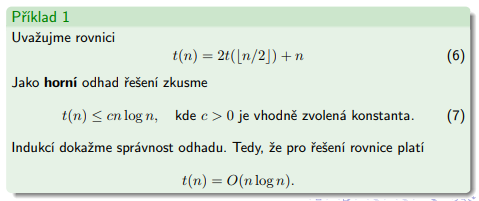
\includegraphics[width=\textwidth, center]{topics/bi-spol-32/images/ind1.PNG}
\end{figure}

\begin{figure}[h]
    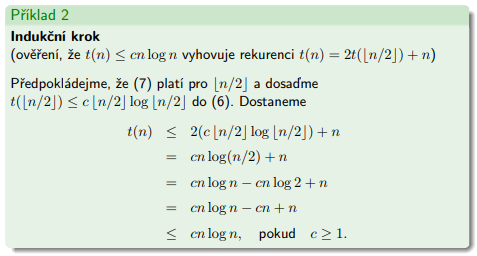
\includegraphics[width=\textwidth, center]{topics/bi-spol-32/images/ind2.PNG}
\end{figure}

\newpage
\subsection{Iterační metoda}

\begin{itemize}
    \item Expandujeme rovnici dle iterací a získáme rozvoj na konečnou řadu a zkusíme najt aritmetickou či geometrickou posloupnost
    \item Využívá se k odhadu horní a dolní meze
\end{itemize}


\begin{figure}[h]
    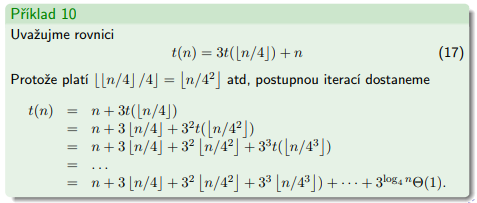
\includegraphics[width=\textwidth, center]{topics/bi-spol-32/images/it1.PNG}
\end{figure}


\begin{figure}[h]
    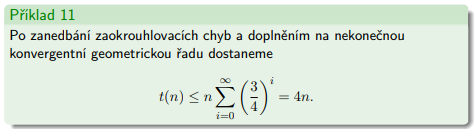
\includegraphics[width=\textwidth, center]{topics/bi-spol-32/images/it2.PNG}
\end{figure}


\subsection{Mistrovská metoda}

Nech $a \geq 1 a b > 1$ jsou konstanty, $f(n)$ funkce jedné proměnné.
Uvažujme rekurentní rovnici: (zanedbáváme ceil a floor)
\begin{center}
    $t(n) = at(n/b) + f(n)$ 
\end{center}

Pak $t(n)$ má následující řešení:
\begin{itemize}
    \item Pokud $f(n) = O(n^{\text{log}_b a - \epsilon} )$ pro nějakou konstantu $\epsilon > 0$, pak $t(n) = \Theta (n^{\text{log}_b a})$.
    \item Pokud $f(n) = \Theta (n^{\text{log}_b a})$, pak $t(n) = \Theta (n^{\text{log}_b a} \text{log} n)$.
    \item Pokud $f(n) = \Omega (n^{\text{log}_b a + \epsilon} )$ pro nějakou konstantu $\epsilon > 0$ a pokud
    $af(n/b)~\leq~cf(n)$ pro nějakou konstantu $c < 1$ a všechna $n \geq n_0$, pak $t(n) = \Theta (f(n))$.
    \item Pokud je rozdíl mezi funkcemi menší než polynomiální, nelze tuto metodu použít!
\end{itemize}



\begin{figure}[h]
    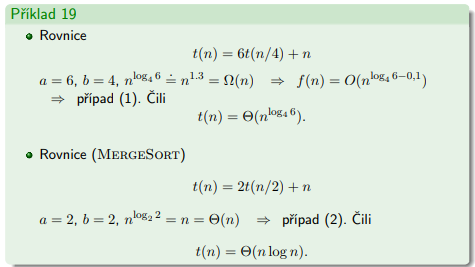
\includegraphics[width=\textwidth, center]{topics/bi-spol-32/images/mt1.PNG}
\end{figure}

\begin{figure}[h]
    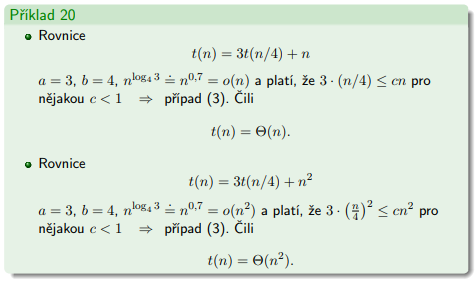
\includegraphics[width=\textwidth, center]{topics/bi-spol-32/images/mt2.PNG}
\end{figure}

\begin{figure}[h]
    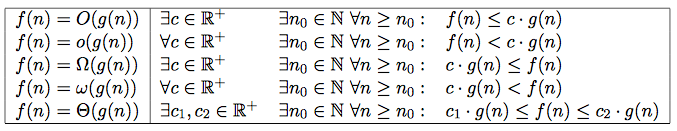
\includegraphics[width=\textwidth, center]{topics/bi-spol-32/images/slozitost.png}
\end{figure}

% \newpage
% \section{Kuchař}

\begin{figure}[h]
    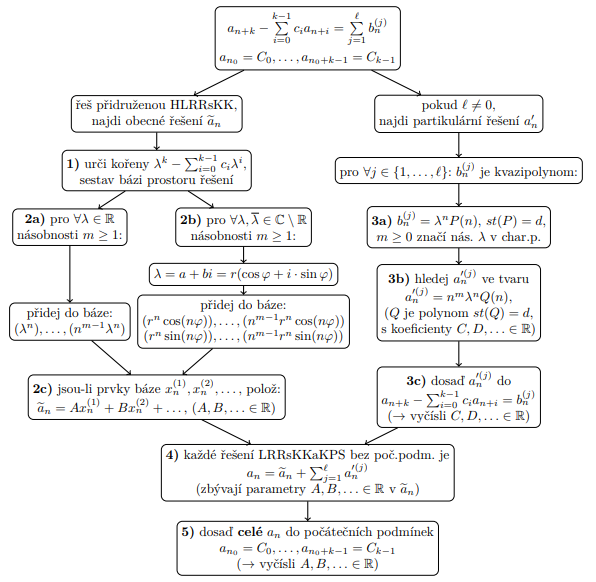
\includegraphics[width=1\textwidth, center]{topics/bi-spol-32/images/kuchar.PNG}
\end{figure}
    

\end{document}
